Ниже (см. магнетон Бура) доказано соотношение 
\[
  p^M_z = \Gamma_0L_z = m\mu_{\text{Б}},
\]
где $ m $ --- магнитное квантовое число, $ p^M $ --- магнитный момент. Эта
формула говорит о дискретности проекции магнитного момента атома на выделенное
направление $ z $ внешнего магнитного поля.

Попробуем доказать или опровергнуть это утверждение эмпирически. Поставим
вакуумную печь, куда положим атомы, например, серебра. Труба у этой печи будет
столь тонкой, что сформируется узкий атомный пучок. Этот пучок пропускают через
неоднородное 
магнитное поле с существенным градиентом магнитной индукции. 
Индукция магнитного поля $ \mathbf B $ в опыте достаточно велика и направлена
вдоль оси $ z $.

Для создания такого магнитного поля используют магнит с ножевидным полюсным наконечником вблизи которого проходит
атомный пучок (рис. \ref{fig:puchok}, б).

\begin{figure}[h]
  \centering
  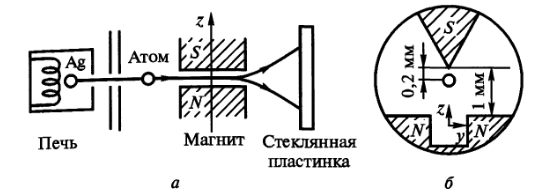
\includegraphics[width=0.8\textwidth]{img/oral-05/puchok.png}
  \label{fig:puchok}
\end{figure}

На пролетающие в зазоре магнита атомы вдоль направления магнитного поля
действует сила  
\[
    F_z = p_z^M \frac{\partial B}{\partial z},
\]
обусловленная градиентом индукции неоднородного магнитного
поля и зависящая от значения проекции магнитного момента 
атома на направление поля. Эта сила отклоняет движущийся атом в
направлении оси $ z $, причем за время пролета магнита движущийся
атом отклоняется тем больше, чем больше сила $ F_z $. При этом одни
атомы отклоняются вверх, а другие --- вниз. Посмотрим на полученную картину на
стеклянной пластинке. Вместо непрерывной зеркальной линии, которая должна была бы
получиться согласно классической физике (ведь тепловое движение хаотично), имеем серию узкиъ зеркальных полосок из
напыленных атомов.

